
\section{Voltage Transfer Curve}

\subsection{Procedure}

For the circuit shown in figure \ref{fig:circuit}, the X-Y mode of the oscilloscope is used to find and display the voltage transfer curve. The value of the resistor is $R=295.3 \Omega$. The power supply uses an over-current protection of $200mA$ and a supply voltage $V_{dd} = 10V$. The function generator uses a sine wave with $V_{offset} = 5V$ and a peak-to-peak voltage $V_{pp} = 10V$. The output frequency is set to $f = 100 Hz$. This acts as $V_{in}$ on the reference circuit from figure \ref{fig:circuit}.

\FloatBarrier

\subsection{Results}
With the X-Axis corresponding to $V_{in}$ and the Y-Axis corresponding to $V_{out}$, the resulting VTC graph is presented in figure \ref{fig:vtc_result}. From this graph, the threshold voltage is $V_{tn}\approx 2.0V$. This is consistent with the provided values in the manufacturer's data sheet that lists the threshold voltage in the range from $0.8 V \le V_{tn} \le 3.0 V$.

The optimal biasing point is when $V_{in} = 2.556 V$. This produces an output voltage of $V_{out} = 4.875 V$.

When the frequency of the AC input signal is lowered from $f=100Hz$ to $f=1 Hz$, the voltage transfer line is no longer continuous when viewed on the oscilloscope. There is only one "dot" which moves back and forth along the same path as the original curve, but very slowly. The only reason the curve at $100 Hz$ appears to be continuous is because the "dot" moves back and forth at a very high speed. The "dot" really represents a point $(V_{in},V_{out})$, which oscillates like a sine wave at the prescribed frequency. At $1 Hz$, the dot moves slowly enough to observe its motion, but appears to just be a continuous curve at $100 Hz$.

\FloatBarrier
\begin{figure}[h!]
	\centering
	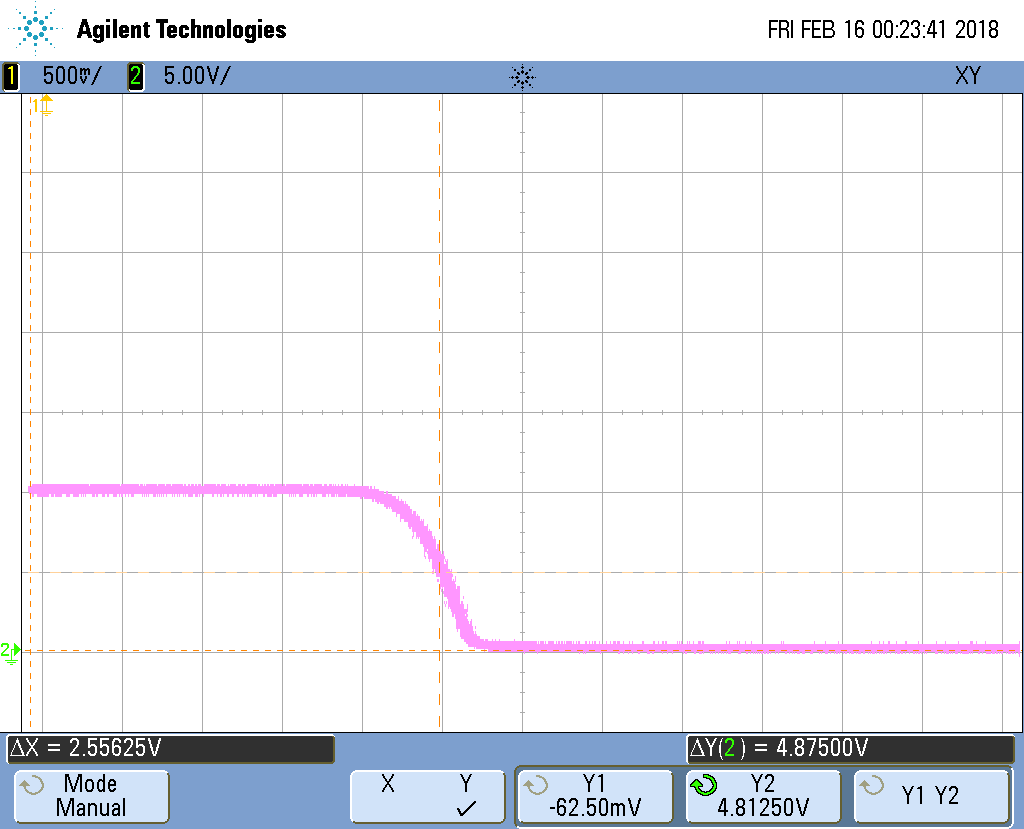
\includegraphics[scale=0.40]{./images/scope_0}
	\caption{Oscilloscope Output for Voltage Transfer Curve Figure \ref{fig:circuit} Circuit}
	\label{fig:vtc_result}
\end{figure}
\FloatBarrier
